\documentclass{article}
% NeurIPS LaTeX style, preprint mode (not an accepted or submitted NeurIPS paper).
\usepackage[preprint]{neurips_2025}
\usepackage[utf8]{inputenc}
\usepackage[T1]{fontenc}
\usepackage{microtype}
\usepackage{graphicx}
\graphicspath{{figures/}}
\usepackage{booktabs}
\usepackage{amsmath}
\usepackage{amsfonts}
\usepackage{nicefrac}
\usepackage{xcolor}
\usepackage{url}
\usepackage[hidelinks]{hyperref}
\setcitestyle{numbers,square}
\usepackage[font=small,labelfont=bf,skip=6pt]{caption}
\usepackage{placeins}
% Breathing room around floats and inside tables
\setlength{\textfloatsep}{16pt plus 4pt minus 2pt}
\setlength{\floatsep}{14pt plus 4pt minus 2pt}
\setlength{\intextsep}{14pt plus 4pt minus 2pt}
\renewcommand{\arraystretch}{1.15}

\title{Illustrated NeurIPS: A Navigable Map of 30{,}225 NeurIPS Papers (2020--2026) with Linked arXiv Records, Citations and Landmark Papers}
\author{%
  Vincent Chu\\
  University of Michigan\\
  \texttt{vcx@umich.edu}
}

\begin{document}
\maketitle

\begin{abstract}
NeurIPS accepted 1{,}898 papers in 2020 and 9{,}111 in 2026. At that volume, reading the proceedings is no longer how researchers learn the shape of the field. We present \emph{Illustrated NeurIPS}, an open dataset and browser-based map of all 30{,}225 papers accepted to NeurIPS from 2020 to 2026. Each paper is embedded from its title and abstract, placed on a two-dimensional map, and assigned to one of 285 fine topics nested in 30 areas, each with a short name and one-sentence description. We link 21{,}946 papers (72.6\%) to their arXiv records, attach citation counts to 26{,}172, and add 1{,}035 highly cited ``landmark'' papers from other venues to the topics they belong to. Against NeurIPS's own subject-area labels, our two-stage clustering (k-means on UMAP features) agrees better than k-means on the raw embeddings (adjusted Rand index 0.086 vs.\ 0.065; paired-bootstrap 95\% interval of the gain $[0.018, 0.023]$) and much better than TF-IDF clustering (0.056). Title-only search over the deployed embeddings retrieves the correct paper first 83.2\% of the time among 26{,}632 abstracts (MRR 0.876, vs.\ 0.761 for TF-IDF). The map shows, for example, that \emph{LLM agent benchmarks} and \emph{RL with verifiable rewards} went from no NeurIPS papers in 2020--21 to 1.5\% and 1.1\% of 2025--26 papers, while \emph{generative adversarial networks} fell from 1.0\% to 0.01\%. The site, data and code are public.
\end{abstract}



\section{Introduction}
NeurIPS has grown nearly fivefold in six years (Figure~\ref{fig:years}). The official proceedings are a list; the conference's own subject labels are coarse (156 distinct labels, 30 top-level areas) and are only published for some years. Tools such as Semantic Scholar~\cite{kinney2023s2} and OpenAlex~\cite{priem2022openalex} index papers individually but do not show how one conference's research is organised or how that organisation changes year to year.

We built a map for that purpose. Our contributions are:
\begin{enumerate}
  \item \textbf{A dataset} of every NeurIPS paper from 2020 to 2026 (main track, Datasets \& Benchmarks, position and journal-track papers) with abstracts, a 384-dimensional embedding, 2D coordinates, a fine and coarse topic with human-readable names, matched arXiv identifiers, primary categories and first-posted dates, citation counts, and ten nearest neighbours.
  \item \textbf{Landmark papers}: 1{,}035 highly cited papers from ICLR, ICML, CVPR, arXiv and elsewhere, admitted to a topic only if the embedding places them inside it, so each NeurIPS topic sits next to the outside work it builds on.
  \item \textbf{An evaluation} of the topic structure against NeurIPS's own labels, with baselines and paired-bootstrap intervals, an evaluation of title-to-paper search, and an independent-model check of topic fit and arXiv matches with a wrong-topic control.
  \item \textbf{A public, client-side tool} (\url{https://vincentychu.com/neurips/}) with semantic search running in the browser, a static JSON API for agents, and per-topic trends.
\end{enumerate}



\begin{figure}[t]
\centering
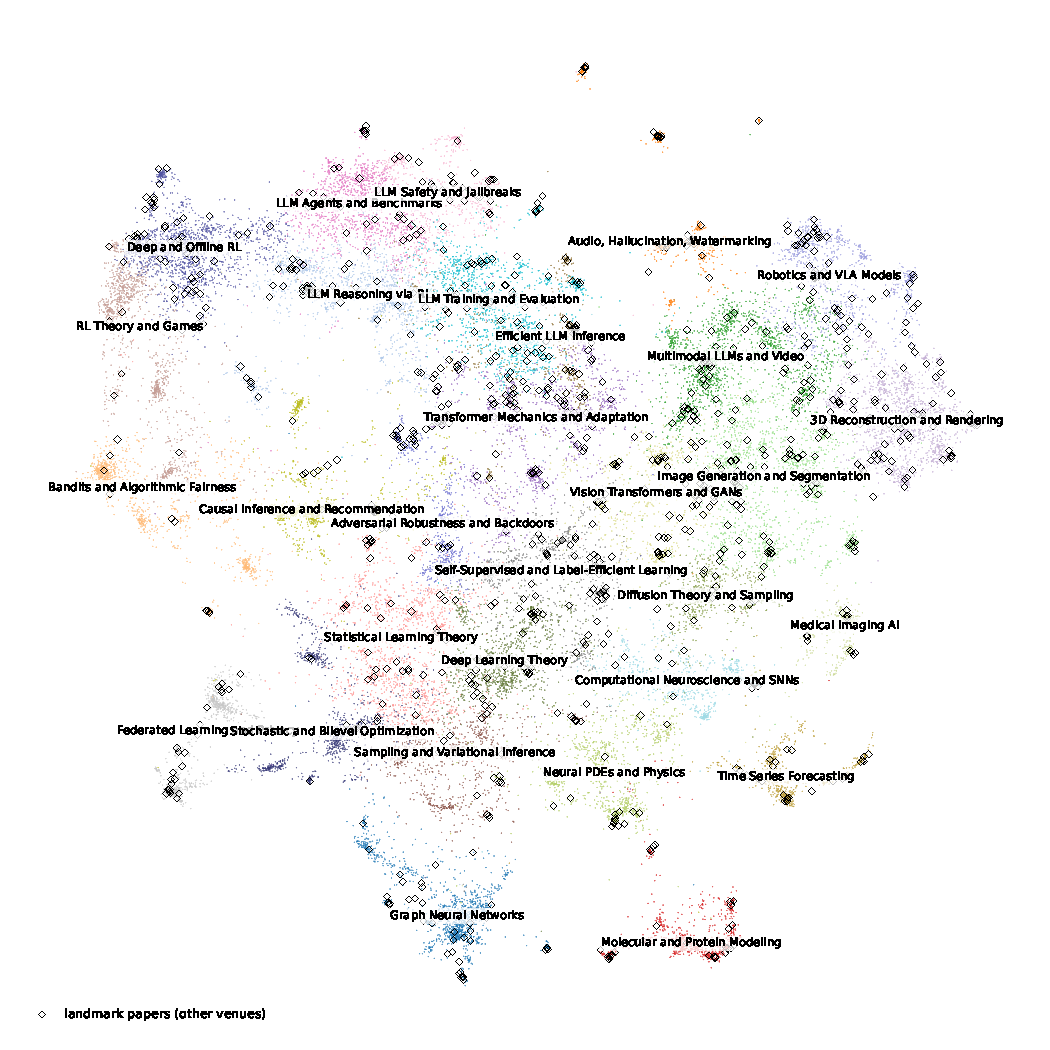
\includegraphics[width=0.82\linewidth]{fig_map.pdf}
\caption{\textbf{Illustrated NeurIPS.} The map: 30{,}225 NeurIPS papers (2020--2026) coloured by area, with area names at their medians. Diamonds are landmark papers from other venues placed in the topics they belong to.}
\label{fig:map}
\end{figure}

\section{Related work}
\textbf{Science maps and topic models.} Topic models such as LDA~\cite{blei2003lda} and, more recently, embedding-plus-clustering pipelines such as BERTopic~\cite{grootendorst2022bertopic} recover themes from document collections. Our pipeline follows the embedding-plus-clustering pattern, with two changes for a navigable map: clustering on a mix of 10D and 2D UMAP features so that topics are contiguous regions of the map people look at, and a second, hierarchical level built on topic centroids.

\textbf{Scholarly metadata.} arXiv's metadata has been studied as a dataset in its own right~\cite{clement2019arxiv}. We use the arXiv API to recover abstracts for papers whose camera-ready versions are not yet public, and Semantic Scholar~\cite{kinney2023s2} and OpenAlex~\cite{priem2022openalex} for citations and landmark candidates.

\textbf{Embeddings for retrieval.} Sentence embeddings~\cite{reimers2019sbert} make semantic search over abstracts cheap. We use bge-small-en-v1.5~\cite{xiao2023cpack} because it is small enough to run in a browser, so that a user's query and the map are embedded by the same model.

\section{Data}
\subsection{Corpus}
We take accepted papers from the conference's public listings (\url{https://neurips.cc/static/virtual/data/neurips-<year>-orals-posters.json}) for 2020--2026, keeping one record per poster (every accepted paper has one) and marking orals and spotlights. The result is 30{,}225 papers: 27{,}042 posters, 2{,}649 spotlights and 534 orals; 27{,}384 main-track, 2{,}411 Datasets \& Benchmarks, 253 journal-track and 177 position papers. Table~\ref{tab:corpus} gives yearly counts.

The listings include abstracts for 2020--2025. For 2026, camera-ready papers were still private on OpenReview when we built the dataset, so we take abstracts from matched arXiv records (5{,}519 papers). The remaining 3{,}592 2026 papers, and one 2025 paper, have titles only and are embedded from their titles.

\begin{table}[t]
\centering\small
\caption{Corpus by year. Subject labels come from the conference listings and exist only for 2023--2026; we use them only for evaluation.}
\label{tab:corpus}
\begin{tabular}{lrrrrrrrr}
\toprule
 & 2020 & 2021 & 2022 & 2023 & 2024 & 2025 & 2026 & Total \\
\midrule
Papers & 1{,}898 & 2{,}334 & 2{,}902 & 3{,}584 & 4{,}538 & 5{,}858 & 9{,}111 & 30{,}225 \\
arXiv match (\%) & 81.4 & 76.9 & 76.9 & 77.1 & 78.8 & 77.1 & 60.6 & 72.6 \\
NeurIPS subject label & -- & -- & -- & 3{,}405 & 4{,}092 & 5{,}504 & 7{,}605 & 20{,}606 \\
\bottomrule
\end{tabular}
\end{table}

\begin{figure}[tbp]
\centering
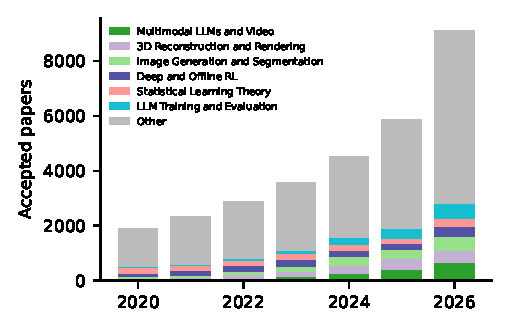
\includegraphics[width=0.5\linewidth]{fig_years.pdf}
\caption{Accepted papers per year, split by the six largest areas.}
\label{fig:years}
\end{figure}

\subsection{arXiv matching}
We query the arXiv API with batches of 100 title phrases. A candidate counts as a match if its normalised title (lower-case letters and digits) equals the paper's, or has a sequence-similarity ratio above 0.92, \emph{and} it was first posted between January of the conference year minus two and December of the conference year plus one. The date window removes title collisions with older or newer papers. We record the arXiv identifier, primary category, first-posted date and abstract. Overall 21{,}946 papers (72.6\%) match; the lower 2026 rate reflects papers not yet posted. We estimate match precision with an independent model in Section~\ref{sec:check}.

\subsection{Citations}
Citation counts come from two sources: OpenAlex works whose primary source is NeurIPS, matched by normalised title and year ($\pm1$), which covers 16{,}979 papers; and Semantic Scholar's batch endpoint for every paper with an arXiv identifier (21{,}946), which also counts citations to the arXiv version. We keep the larger count. 26{,}172 papers have at least one source and 22{,}130 have one or more citations (median over papers with a source: 9). Counts are a snapshot from November 2026, so recent papers are naturally low.

\FloatBarrier
\section{Method}
\subsection{Embedding and layout}
Each paper is embedded as \emph{title}\texttt{. }\emph{abstract} with bge-small-en-v1.5 (CLS pooling, unit-normalised, 384 dimensions). We fit two UMAP~\cite{mcinnes2018umap} projections with cosine distance and 30 neighbours: a 2D layout for display (minimum distance 0.05) and a 10D projection for clustering (minimum distance 0). We also store each paper's ten nearest neighbours by cosine similarity in the full embedding space.

\subsection{Two-level topics}
\textbf{Fine topics.} We run k-means ($k=300$, 4 restarts) on the concatenation of the 10D projection and the 2D layout scaled by 4. The 2D term makes topics contiguous on the displayed map, so a topic is a region a reader can point at. Clusters with fewer than 12 papers are merged into the nearest larger cluster, giving 285 fine topics (median 89 papers; range 13--414).

\textbf{Areas.} We group fine topics into 30 areas with Ward agglomerative clustering on topic centroids, where each centroid concatenates the mean embedding (scaled by 3) and the mean 2D position (scaled by 4).

\textbf{Names and descriptions.} For each topic we compute distinctive terms (TF-IDF over titles and abstracts, unigrams and bigrams, divided by the term's corpus-wide mean), the ten titles closest to the topic's mean embedding, and its paper count per year. A language model (Claude, run headless in batches of 30 topics) returns a 2--5 word name and a one-sentence description that may note the trend in the yearly counts, under the constraint that names be specific and distinct. Keyword names are the fallback when no name is returned. For example: \emph{Computational Social Choice} (``Voting rules, distortion bounds, peer prediction, sortition and fair allocation mechanisms\ldots'') and \emph{Surrogate Loss Consistency} (``Studies H-consistency and Bayes-consistency of surrogate losses\ldots'').

\subsection{Landmark papers}
For each fine topic we query Semantic Scholar's bulk search with the topic's five most distinctive terms, sorted by citation count, restricted to 2020--2026 and at least 40 citations, and keep up to 80 candidates with abstracts. We drop NeurIPS papers and papers already in the corpus. A candidate is admitted to a topic only if (i) its embedding's nearest topic centroid is that topic and (ii) its similarity to that centroid is at least the 25th percentile of the topic's own members. Within each topic we keep at most eight, ranked by citations per year since publication, and place them on the map with the fitted UMAP transform. This yields 1{,}035 landmarks in 213 of the 285 topics (median 779 citations), led by arXiv-only papers (133), ICLR (127), CVPR (123) and ICML (110).

\subsection{The tool}
The site is static. The browser downloads the map (coordinates, topics, metadata), per-year abstract files and an int8-quantised copy of the embeddings (12\,MB for all papers and landmarks). Search embeds the query in the browser with the same model (quantised, via Transformers.js), with bge's retrieval instruction prepended to queries, and ranks papers by cosine similarity. A pasted arXiv link is fetched, embedded and placed on the map. Each topic page shows its description, yearly counts, most-cited papers per year and landmarks. A static JSON API (topic and paper files) lets software agents use the same data.

\FloatBarrier
\section{Evaluation}
\subsection{Agreement with NeurIPS subject labels}
For 2023--2026 the conference listings carry an author-selected subject label for 20{,}606 papers. Labels appear in two formats across years (``A->B'' and ``A/B''); after normalising, there are 156 distinct fine labels and 30 top-level areas. These labels are coarse and self-reported, so they are a noisy reference, not ground truth; we use them to compare methods on the same data, not to measure absolute quality.

We compare our fine topics and areas with (a) k-means with the same $k$ on the raw 384D embeddings (three seeds), (b) k-means on a 256-dimensional LSA projection of TF-IDF vectors of title and abstract, and (c) random assignment. We report normalised mutual information (NMI)~\cite{strehl2002cluster} and the adjusted Rand index (ARI)~\cite{hubert1985ari}, fine topics against fine labels and areas against top-level labels.

\begin{table}[t]
\centering\footnotesize\setlength{\tabcolsep}{4pt}
\caption{Agreement with NeurIPS subject labels on 20{,}606 papers (2023--2026): 285 fine topics vs.\ 156 fine labels, and 30 areas vs.\ 30 top-level labels. Bootstrap: 300 resamples of labelled papers.}
\label{tab:cluster}
\begin{tabular}{lcccc}
\toprule
 & \multicolumn{2}{c}{Fine topics} & \multicolumn{2}{c}{Areas} \\
\cmidrule(lr){2-3}\cmidrule(lr){4-5}
Method & NMI & ARI & NMI & ARI \\
\midrule
Random & 0.146 & 0.000 & 0.007 & 0.000 \\
TF-IDF + LSA + k-means & 0.377 & 0.056 & 0.230 & 0.076 \\
k-means, embeddings (seed 0) & 0.415 & 0.065 & 0.262 & 0.094 \\
k-means, embeddings (seeds 1, 2) & 0.413, 0.412 & 0.064, 0.067 & 0.261, 0.263 & 0.102, 0.104 \\
\textbf{Ours} (UMAP k-means, Ward) & \textbf{0.425} & \textbf{0.086} & \textbf{0.267} & \textbf{0.110} \\
\midrule
Ours $-$ k-means s0, mean & +0.009 & +0.020 & +0.005 & +0.016 \\
\quad 95\% paired-bootstrap interval & [0.006, 0.011] & [0.018, 0.023] & [0.002, 0.009] & [0.013, 0.019] \\
\bottomrule
\end{tabular}
\end{table}

Table~\ref{tab:cluster} shows that our clustering agrees with the conference's labels more than k-means on the same embeddings for every metric and level, and the paired-bootstrap intervals exclude zero. The gain is modest in NMI and larger in ARI (about a third, relative, at the fine level), consistent with UMAP features producing tighter, more balanced groups. Seed variation of the baseline (ARI 0.064--0.067 at the fine level) is far smaller than the gap. Embeddings beat TF-IDF by a wide margin. Absolute values are low for all methods because 285 data-driven topics and 156 broad, self-chosen labels slice the field differently; for instance, our clustering separates ``LLM-as-a-Judge Evaluation'' from ``LLM Agent Benchmarks'', which share a NeurIPS label.

\subsection{Search}
We sample 2{,}000 papers with abstracts, use each \emph{title alone} as the query, and rank all 26{,}632 papers with abstracts by similarity to their \emph{abstract only}, so the query text never appears in the document. Table~\ref{tab:search} reports the rank of the source paper.

\begin{table}[t]
\centering\small
\caption{Title-to-abstract retrieval over 26{,}632 abstracts (2{,}000 queries).}
\label{tab:search}
\begin{tabular}{lcccc}
\toprule
Query encoding & MRR & R@1 & R@10 & R@100 \\
\midrule
TF-IDF (cosine) & 0.761 & 0.686 & 0.892 & 0.970 \\
bge-small, plain query & 0.833 & 0.774 & 0.934 & 0.984 \\
bge-small + TF-IDF, z-score sum & 0.830 & 0.769 & 0.940 & 0.990 \\
\textbf{bge-small with retrieval instruction (deployed)} & \textbf{0.876} & \textbf{0.832} & \textbf{0.949} & 0.988 \\
\bottomrule
\end{tabular}
\end{table}

The deployed setting, which prepends bge's retrieval instruction to the query, finds the right paper first 83.2\% of the time and in the top 10 for 94.9\%. A simple hybrid with TF-IDF did not help.

\subsection{Topic-fit and arXiv-match check}
\label{sec:check}
We drew a stratified random sample of 150 papers with abstracts (proportional by year) and 50 arXiv-matched papers from 2020--2025. Because the topic names were written by one language model (Claude), we used a \emph{different} model, GLM-5.3-Flash run locally, as an independent judge, so that no model grades its own output. For each sampled paper the judge saw the title, abstract and the assigned topic's name and description and answered yes, partly (related, but the topic misses the main contribution) or no. For each arXiv match it saw both abstracts and judged whether they describe the same paper. As a control, we showed the judge 50 sampled papers with a randomly chosen \emph{wrong} topic.

\begin{table}[t]
\centering\small
\caption{Independent LLM-judge check (GLM-5.3-Flash) and the author's check of a subset. Wilson 95\% intervals: topic fits fully 52.0--67.5\%, at least partly 80.3--91.2\%; arXiv precision 92.9--100\%.}
\label{tab:judge}
\begin{tabular}{lrrr}
\toprule
Check & Yes & Partly & No \\
\midrule
Assigned topic fits the paper ($n=150$) & 90 (60.0\%) & 40 (26.7\%) & 20 (13.3\%) \\
Control: random wrong topic ($n=50$) & 2 (4.0\%) & 2 (4.0\%) & 46 (92.0\%) \\
arXiv record is the same paper ($n=50$) & 50 (100\%) & 0 & 0 \\
\midrule
Author, assigned topic fits ($n=73$, subset) & 32 (43.8\%) & 29 (39.7\%) & 12 (16.4\%) \\
LLM judge on the same 73 papers & 47 (64.4\%) & 18 (24.7\%) & 8 (11.0\%) \\
\bottomrule
\end{tabular}
\end{table}

Table~\ref{tab:judge} shows the judge separates assigned from random topics sharply (92\% of wrong topics rejected), so its verdicts carry signal. The assigned topic fits fully for 60\% of papers and at least partly for 87\%. Most ``partly'' cases are papers at a topic's edge whose main contribution belongs to a neighbouring topic, such as an interpretability benchmark for time-series models placed under time-series forecasting. Every sampled arXiv match was the same paper, so the title-plus-date-window rule appears precise; it cannot measure recall, which is bounded above by the 72.6\% match rate. The author also labelled 73 of the 150 topic items in the released labelling page and is stricter than the judge: the topic fits fully for 43.8\% of these papers (Wilson 95\% interval 33.0--55.2\%) and at least partly for 83.6\% (73.4--90.3\%), against 64.4\% and 89.0\% from the judge on the same papers. The two agree exactly on 53.4\% of items (Cohen's $\kappa = 0.23$) and on whether the topic fits at all on 83.6\%. We therefore read the judge's 60\% full-fit rate as an upper estimate. The judge's verdicts, the author's labels and the labelling page are released so others can repeat the check.

\FloatBarrier
\section{What the map shows}
Comparing each topic's share of papers in 2020--21 with 2025--26 gives a compact picture of how NeurIPS changed (Table~\ref{tab:trends}). The fastest-growing topics did not exist at NeurIPS five years earlier and are all about large language models used as agents, judges or reasoners. The steepest declines are in topics that were central in 2020: GANs, adversarial robustness, pruning and meta-learning. Because topics are defined by content rather than labels, these trends can be read directly off the map and the per-topic year charts.

\begin{table}[h]
\centering\small
\caption{Largest risers and fallers by share of NeurIPS papers, 2020--21 vs.\ 2025--26 (topics with at least 40 papers, or 30 in 2020--21 for fallers).}
\label{tab:trends}
\begin{tabular}{lrrrr}
\toprule
Topic & \multicolumn{2}{c}{Papers} & \multicolumn{2}{c}{Share (\%)} \\ & 2020--21 & 2025--26 & 2020--21 & 2025--26 \\
\midrule
LLM Agent Benchmarks & 0 & 224 & 0.00 & 1.50 \\
RL with Verifiable Rewards & 0 & 167 & 0.00 & 1.12 \\
AI Scientists, Agents and Debate & 0 & 123 & 0.00 & 0.82 \\
LLM Agent Security & 0 & 114 & 0.00 & 0.76 \\
LLM-as-a-Judge Evaluation & 0 & 104 & 0.00 & 0.69 \\
\midrule
Generative Adversarial Networks & 43 & 2 & 1.02 & 0.01 \\
Adversarial Robustness & 95 & 25 & 2.24 & 0.17 \\
Network Pruning and Lottery Tickets & 39 & 12 & 0.92 & 0.08 \\
Meta-Learning & 47 & 18 & 1.11 & 0.12 \\
\bottomrule
\end{tabular}
\end{table}





\section{Limitations}
2026 papers are under-described: 3{,}592 have titles only, and 39.4\% have no arXiv match, so their placement and topics are less reliable. Topic names come from a language model given keywords and representative titles and can be too narrow for papers at a topic's edge: an independent model judged the assigned topic a full fit for 60\% of sampled papers and a partial fit for another 27\%. The author's check of 73 of these papers was stricter (43.8\% full fit, 83.6\% at least partial), so the true full-fit rate is likely lower than the judge's. NeurIPS subject labels are self-reported and coarse, so agreement with them is a relative, not absolute, measure. Citation counts are a single snapshot and favour older papers. Landmark candidates are limited to what Semantic Scholar's keyword search returns for each topic's terms, so a topic with unusual vocabulary may have none (72 of 285 topics do not). UMAP layouts and k-means depend on random seeds; we fixed seeds and report baseline seed variance, but did not re-run the full pipeline across seeds.

\section{Availability}
\begin{itemize}
  \item Interactive map: \url{https://vincentychu.com/neurips/} (data files, static API and agent instructions are served under the same path).
  \item Code and evaluation: \url{https://github.com/vinceychu/illustrated-neurips}, under \texttt{scripts/neurips/} (corpus assembly, arXiv matching, citations, embedding, layout, naming, landmarks, export) and \texttt{paper/} (this paper and its evaluation).
  \item Archived (all versions): \href{https://doi.org/10.5281/zenodo.24301136}{doi:10.5281/zenodo.24301136}.
\end{itemize}

\begin{thebibliography}{12}
\bibitem[Blei et~al.(2003)]{blei2003lda} D.~M. Blei, A.~Y. Ng, and M.~I. Jordan. Latent Dirichlet allocation. \emph{Journal of Machine Learning Research}, 3:993--1022, 2003.
\bibitem[Clement et~al.(2019)]{clement2019arxiv} C.~B. Clement, M.~Bierbaum, K.~P. O'Keeffe, and A.~A. Alemi. On the use of arXiv as a dataset. \emph{arXiv:1905.00075}, 2019.
\bibitem[Grootendorst(2022)]{grootendorst2022bertopic} M.~Grootendorst. BERTopic: Neural topic modeling with a class-based TF-IDF procedure. \emph{arXiv:2203.05794}, 2022.
\bibitem[Hubert and Arabie(1985)]{hubert1985ari} L.~Hubert and P.~Arabie. Comparing partitions. \emph{Journal of Classification}, 2(1):193--218, 1985.
\bibitem[Kinney et~al.(2023)]{kinney2023s2} R.~Kinney et~al. The Semantic Scholar open data platform. \emph{arXiv:2301.10140}, 2023.
\bibitem[McInnes et~al.(2018)]{mcinnes2018umap} L.~McInnes, J.~Healy, and J.~Melville. UMAP: Uniform manifold approximation and projection for dimension reduction. \emph{arXiv:1802.03426}, 2018.
\bibitem[Priem et~al.(2022)]{priem2022openalex} J.~Priem, H.~Piwowar, and R.~Orr. OpenAlex: A fully-open index of scholarly works, authors, venues, institutions, and concepts. \emph{arXiv:2205.01833}, 2022.
\bibitem[Reimers and Gurevych(2019)]{reimers2019sbert} N.~Reimers and I.~Gurevych. Sentence-BERT: Sentence embeddings using Siamese BERT-networks. In \emph{Proceedings of EMNLP-IJCNLP}, 2019.
\bibitem[Strehl and Ghosh(2002)]{strehl2002cluster} A.~Strehl and J.~Ghosh. Cluster ensembles: A knowledge reuse framework for combining multiple partitions. \emph{Journal of Machine Learning Research}, 3:583--617, 2002.
\bibitem[Xiao et~al.(2023)]{xiao2023cpack} S.~Xiao, Z.~Liu, P.~Zhang, and N.~Muennighoff. C-Pack: Packaged resources to advance general Chinese embedding. \emph{arXiv:2309.07597}, 2023.
\end{thebibliography}

\end{document}
